%% TODO:
%% would it be better to just talk about permutations here? and observe that
%% paths through the interior are equivalent to paths on the perimeter?
%% then put this section in the JPS chapter?

\section{Path Symmetries}
Pathfinding in modern video games often involves exploring environments such
as cities, sewers or dungeons. Often represented using a grid map, these
locales tend to be topographically simple (e.g. empty rooms, connected by
corridors) but can be surprisingly difficult to search.  This is because
between any pair of locations in a grid map there usually exist many possible
paths. Sometimes these paths represent alternative ways of reaching one
location from the other. More often they are symmetric in the sense that the
only difference between them is the order in which individual moves appear.
Definition~\ref{def::rsr::gridpath} introduces the concept of symmetry more
formally.  As an illustrative example consider
Figure~\ref{fig::rsr::symmetry}.  Suppose we run an optimal algorithm such as
A* to solve this problem.  Each time we expand a node $n$ we need to expand
all nodes on any shortest path to $n$, including all permutations each of which
is also a shortest path to $n$. Depending on how we break ties, we
might expand a majority of all nodes before reaching the goal.

\begin{figure}[tb]
\begin{center}
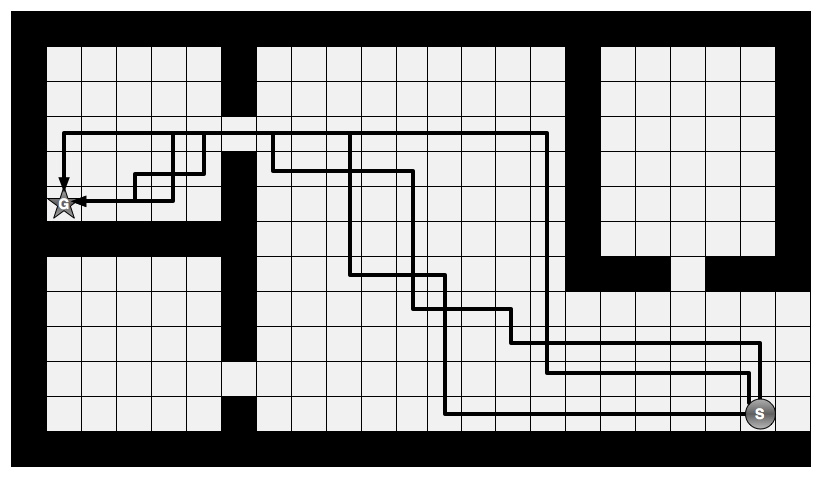
\includegraphics[scale=0.30, trim = 10mm 10mm 10mm 0mm]{chapter_rsr/diagrams/symmetry.png}
\end{center}
\vspace{-3pt}
\caption[An example of path symmetry]{
\small
A pathfinding instance on a 4-connected grid map. There are many optimal
paths between the start and target location but all are permutations of 
one another. We highlight three such paths.}

\label{fig::rsr::symmetry}
\end{figure}

Despite a wealth of research on the topic of symmetry breaking (see
Chapter~\ref{cha::lit::symmetry}) few works deal with the problem in the
context of pathfinding search.  This lack of attention may stem from
definitional issues. For example, researchers commonly define a path as a
sequence of connected edges which together represent a walk in a search graph.
The problem is that edges are strictly ordered whereas the actions they
represent could be pairwise commutative~\citep{haslum00}; i.e. we could apply
the actions in any order and still reach the same state.  To help identify
such situations we introduce a slightly different notion of a path:

\begin{definition}
\label{def::rsr::gridpath}
A \emph{grid path} $\pi = \langle \vec{v_1}, \ldots, \vec{v_k} \rangle$ is an ordered sequence 
of vectors, where each vector $\vec{v_i}$ represents a single step from one node of 
the grid to an adjacent neighbouring node. 
%Straight steps have a cost of 1. Diagonal steps have a cost of $\sqrt{2}$.
\end{definition}

Put more simply Definition~\ref{def::rsr::gridpath} says that a path is just a
a sequence of single steps, or moves, and that each move is a direction on the 
grid such as North, South, East or West. Using
Definition~\ref{def::rsr::gridpath} we can now distinguish between paths that
are merely equivalent (i.e. of the same length) and those that are symmetric:

\begin{definition}
Two grid paths $\pi$ and $\pi'$ are symmetric iff: (i) they share the same 
start and end node (ii) they have the same cost and (iii) one can be derived from 
the other by swapping the order of the constituent vectors.
\end{definition}


